\section{ROC curves}
\label{app:roc}


\begin{figure}[ht]
\centering
\begin{subfigure}[b]{0.45\textwidth}\centering\caption{}
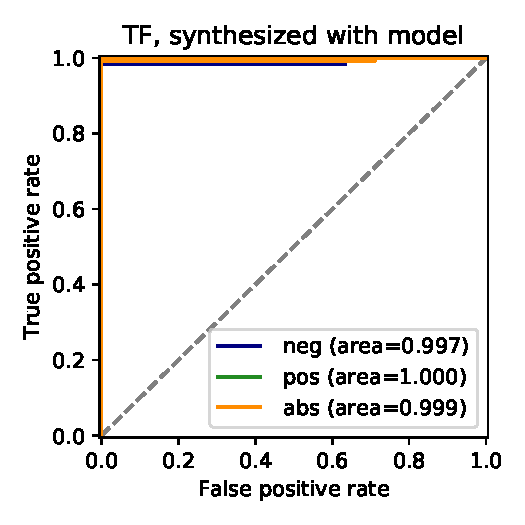
\includegraphics[width=\textwidth]{analysis/fig/roc_tf_prim.pdf}
\end{subfigure}
\hfill
\begin{subfigure}[b]{0.45\textwidth}\centering\caption{}
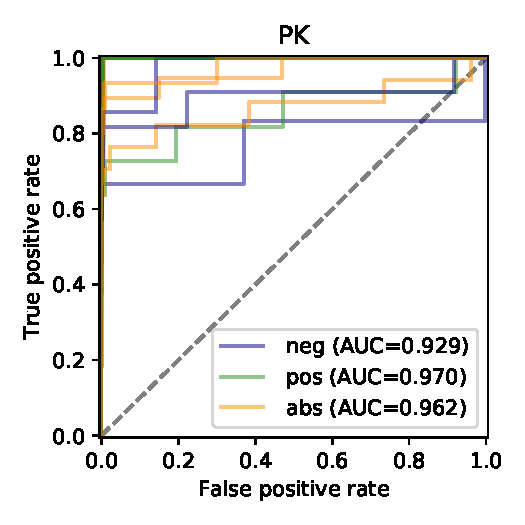
\includegraphics[width=\textwidth]{appendices/fig/roc_pk_prim.pdf}
\end{subfigure}
\vskip\baselineskip
\begin{subfigure}[b]{0.45\textwidth}\centering\caption{}
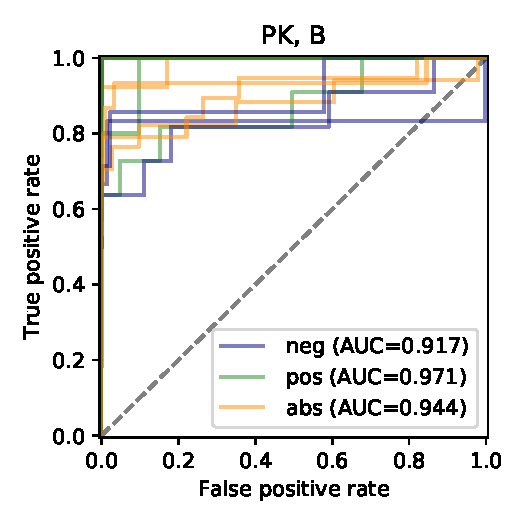
\includegraphics[width=\textwidth]{appendices/fig/roc_pk_prim_B.pdf}
\end{subfigure}
\hfill
\begin{subfigure}[b]{0.45\textwidth}\centering\caption{}
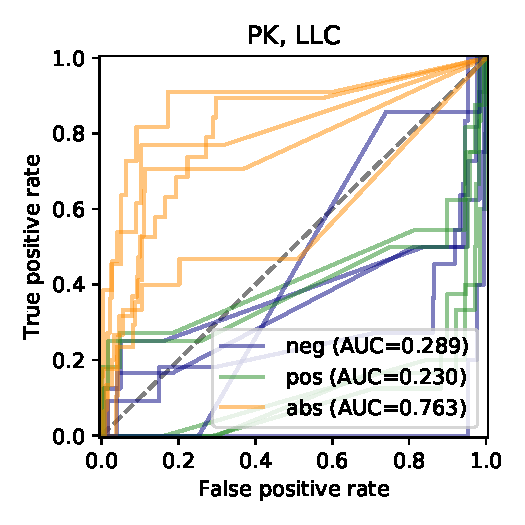
\includegraphics[width=\textwidth]{appendices/fig/roc_pk_prim_llc.pdf}
\end{subfigure} 
\caption{\textbf{ROC curves for inference of edge values on simple simulated data for 5 individual graphs.} ROC curves for each of the individual 5 100-node graphs. Inference on RNA gene expression levels simulated with the same model used for inference. Inference on TF edges~(a), PK edges~(b), PK edges using B method~(c), and on PK edges using the Eberhardt LLC method~(d).}
\label{fig:prim_each}
\end{figure}




\begin{figure}[ht]
\centering
\begin{subfigure}[b]{0.45\textwidth}\centering\caption{}
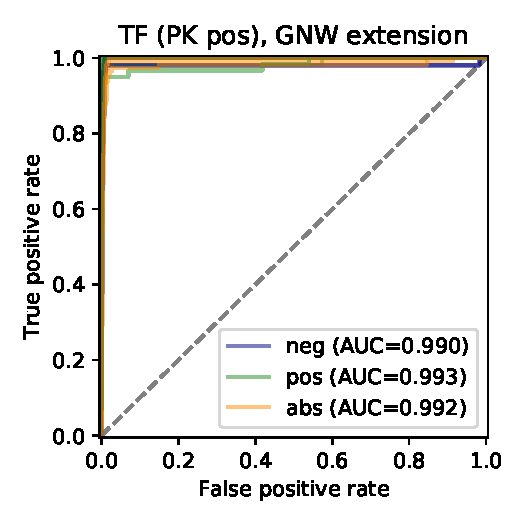
\includegraphics[width=\textwidth]{appendices/fig/roc_tf_gnw_pos_each.pdf}\label{fig:gnw_each.a}
\end{subfigure}
\hfill
\begin{subfigure}[b]{0.45\textwidth}\centering\caption{}
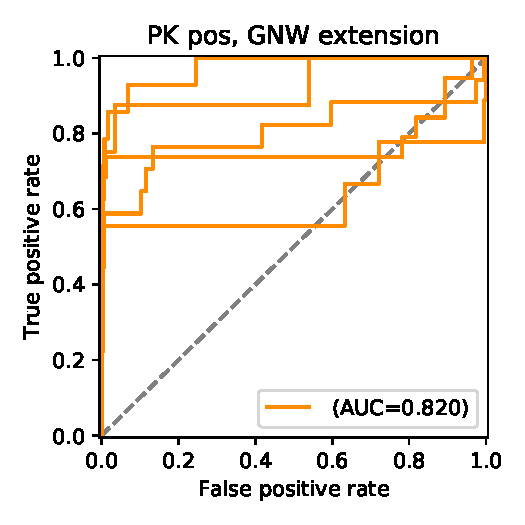
\includegraphics[width=\textwidth]{appendices/fig/roc_pk_gnw_pos.pdf}
\end{subfigure}
\vskip\baselineskip
\begin{subfigure}[b]{0.45\textwidth}\centering\caption{}
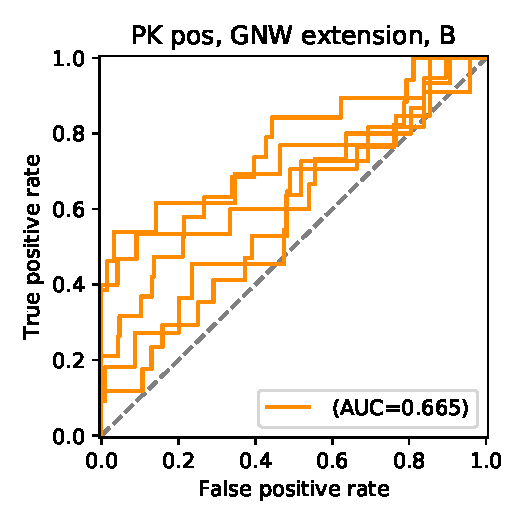
\includegraphics[width=\textwidth]{appendices/fig/roc_pk_gnw_pos_B.pdf}
\end{subfigure}
\hfill
\begin{subfigure}[b]{0.45\textwidth}\centering\caption{}
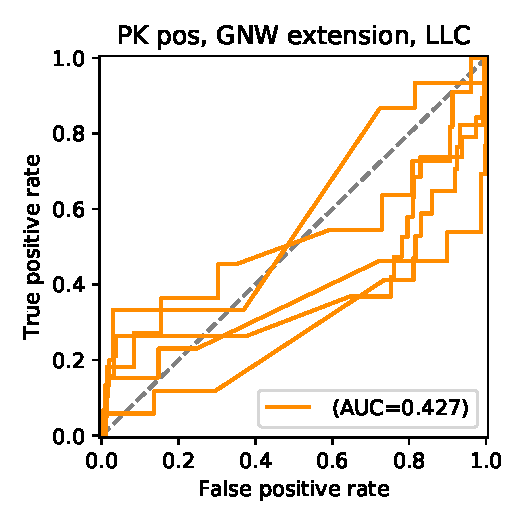
\includegraphics[width=\textwidth]{appendices/fig/roc_pk_gnw_pos_llc.pdf}
\end{subfigure} 
\caption{\textbf{ROC curves for inference of edge values on simulated GNW extension data for 5 individual graphs.} ROC curves for each of the individual 5 100-node graphs. Inference on RNA gene expression levels simulated with the GeneNetWeaver kinase extension. Inference on TF edges~(a), PK edges~(b), PK edges using B method~(c), and on PK edges using the Eberhardt LLC method~(d).}
\label{fig:gnw_each}
\end{figure}





